En esta sección intrucimos el concepto de modelo de lenguage. Un enfoque de asignar probabilidades a oraciones que como veremos a lo largo del apunte cumplirá un rol fundamental en enfoquemos modernos de PLN.


\section{El Problema del Modelado del Lenguaje}

Tenemos un vocabulario (finito), digamos $\mathcal{V} = \{$el, un, hombre, telescopio, Zamorano, dos, fan, vio, jugar, para, Real, Madrid, Zamorano, . . .$\}$, del cual podemos formar n conjunto (infinito) de oraciones, $\mathcal{V}^*$.  Por ejemplo:
\begin{itemize}
\item el STOP
\item un STOP
\item el fan STOP
\item el fan vio a Zamorano STOP
\item el fan vio vio STOP
\item el fan vio a Zamorano jugar por el Real Madrid STOP
\end{itemize}

Donde STOP es un símbolo especial que indica el final de una oración. Tenemos una muestra de entrenamiento de ejemplos de oraciones en inglés. Necesitamos ``aprender'' una distribución de probabilidad $p$. Donde $p$ es una función que satisface:
\begin{align*}
\sum_{x\in V^*} p(x) &= 1 \\
p(x) &\geq 0 \quad \text{para todo } x \in V^*
\end{align*}

Ejemplos de probabilidades asignadas a las oraciones:
\begin{align*}
p(\text{el STOP}) &= 10^{-12} \\
p(\text{el fan STOP}) &= 10^{-8} \\
p(\text{el fan vio a Zamorano STOP}) &= 2 \times 10^{-8} \\
p(\text{el fan vio vio STOP}) &= 10^{-15} \\
\ldots \\
p(\text{el fan vio a Zamorano jugar por el Real Madrid STOP}) &= 2 \times 10^{-9}
\end{align*}

Lo que esperamos del modelo es que le asigne una probabilidad más alta a las oraciones fluidas (aquellas que tienen sentido y son gramaticalmente correctas) de las que no. También esperamos poder estimar esta función de probabilidad a partir del texto (corpus).

A nivel general, el modelo de lenguaje ayuda a los modelos de generación de texto a distinguir entre buenas y malas oraciones.



\subsection{¿Por qué querríamos hacer esto?}

El reconocimiento del habla fue la motivación original. Consideremos las siguientes dos oraciones en inglés:
\begin{enumerate}
 \item ``recognize speech''  (reconocer el habla)
 \item ``wreck a nice beach'' (arruinar una playa bonita).
\end{enumerate}

Estas dos oraciones suenan muy similares al ser pronunciadas, lo que dificulta que los sistemas automáticos de reconocimiento del habla las transcriban con precisión. Cuando el sistema de reconocimiento del habla analiza la entrada de audio e intenta transcribirlo, tiene en cuenta las probabilidades del modelo de lenguaje para determinar la interpretación más probable.
El modelo de lenguaje favorecería $p$(``recognize speech'') sobre $p$(``wreck a nice beach'').
Esto se debe a que la primera oración es más común y debería ocurrir con más frecuencia en el corpus de entrenamiento.

Al incorporar modelos de lenguaje, los sistemas de reconocimiento del habla pueden mejorar  la precisión al seleccionar la oración que se alinea mejor con los patrones lingüísticos y el contexto, incluso cuando se enfrentan a alternativas que suenan similar.

De hecho, los modelos de lenguaje son útiles en cualquier tarea de procesamiento del lenguaje natural que involucre la generación de lenguaje (por ejemplo, traducción automática, resumen, generación de resumenes, chatbots,  reconocimiento óptico de caracteres y el reconocimiento de escritura a mano).

Además la noción de modelamiento probabilistico del lenguaje se utiliza en muchos modelos y tareas de PLN, por lo que las técnicas de estimación desarrolladas en este capítulo serán muy útiles para entender muchos problemas en PLN.


\subsection{Los Modelos de Lenguaje son Generativos}
Los modelos de lenguaje una vez aprendidos a partir de un corpus pueden usarse para generar oraciones nuevas al muestrear secuencialmente a partir de las probabilidades.

Esto es análogo a extraer bolas (palabras) de una urna donde sus tamaños son proporcionales a sus frecuencias relativas.

Alternativamente, uno siempre podría extraer la palabra más probable, lo cual es equivalente a predecir la siguiente palabra.


\subsection{Un Método Ingenuo}
Un método muy ingenuo para estimar la probabilidad de una oración es contar las apariciones de la oración en los datos de entrenamiento y dividirlo por el número total de oraciones de entrenamiento ($N$) para estimar la probabilidad. Tenemos $N$ oraciones de entrenamiento.
Para cualquier oración $x_1, x_2, \ldots, x_n$, $c(x_1, x_2, \ldots, x_n)$ es el número de veces que se ha visto la oración en nuestros datos de entrenamiento. Una estimación ingenua: \begin{displaymath}
p(x_1,x_2,\cdots,x_n)=\frac{c(x_1,x_2 \dots,x_n)}{N}
\end{displaymath}

El problema de este enfoque, es que a medida que el número de posibles oraciones crece de manera exponencial con la longitud de las oraciones y el tamaño del vocabulario, se vuelve cada vez más improbable que una oración específica aparezca en los datos de entrenamiento.

En consecuencia, muchas oraciones tendrán una probabilidad cero según el modelo ingenuo, lo que lleva a una mala generalización.

\section{Procesos de Markov}
Considera una secuencia de variables aleatorias $X_1, X_2, \ldots, X_n$. Cada variable aleatoria puede tomar cualquier valor en un conjunto finito $V$. Por ahora, asumimos que la longitud $n$ está fija (por ejemplo, $n = 100$). Nuestro objetivo: modelar $P(X_1 = x_1, X_2 = x_2, \ldots, X_n = x_n)$

\subsection{Procesos de Markov de primer orden}

Un proceso de Markov de primer orden asume que la probabilidad de que una variable aleatoria tome un valor depende únicamente del valor inmediatamente anterior en la secuencia. En el contexto del modelado del lenguaje, esto significa que la probabilidad de una palabra en una oración depende solo de la palabra anterior. La probabilidad conjunta de una secuencia de palabras se calcula multiplicando las probabilidades condicionales de las palabras sucesivas dado su predecesor inmediato. Esta es la suposición de Markov de primer orden:

\[
P(X_i = x_i|X_1 = x_1, \ldots, X_{i-1} = x_{i-1}) = P(X_i = x_i|X_{i-1} = x_{i-1})
\]

\subsection{Procesos de Markov de segundo orden}

Un proceso de Markov de segundo orden amplía la suposición de Markov de primer orden y considera el valor de dos variables anteriores en la secuencia. En el modelado del lenguaje, esto significa que la probabilidad de una palabra en una oración depende de las dos palabras anteriores. La probabilidad conjunta de una secuencia de palabras se calcula multiplicando las probabilidades condicionales de las palabras sucesivas dado sus dos predecesores inmediatos. La suposición de Markov de segundo orden es la siguiente:

\[
P(X_i = x_i|X_1 = x_1, \ldots, X_{i-2} = x_{i-2}, X_{i-1} = x_{i-1}) = P(X_i = x_i|X_{i-2} = x_{i-2}, X_{i-1} = x_{i-1})
\]

\subsection{Modelado de secuencias de longitud variable}

Si queremos modelar secuencias de longitud variable, podemos considerar que la longitud de la secuencia, $n$, también es una variable aleatoria. Una forma simple de abordar esto es siempre definir $X_n = \text{STOP}$, donde "STOP" es un símbolo especial que marca el final de la secuencia. Luego, podemos usar un proceso de Markov como antes para modelar la probabilidad conjunta de las palabras en la secuencia:

\[
P(X_1 = x_1, X_2 = x_2, \ldots, X_n = x_n) = \prod_{i=1}^{n} P(X_i = x_i|X_{i-2} = x_{i-2}, X_{i-1} = x_{i-1})
\]

Aquí, asumimos que $x_0 = x_{-1} = *$ por conveniencia, donde "*" es un símbolo especial de "inicio".

\section{Modelos de lenguaje trigram}

Un modelo de lenguaje trigram consiste en:

\begin{enumerate}
  \item Un conjunto finito $V$ de palabras.
  \item Un parámetro $q(w|u, v)$ para cada trigram $u, v, w$ donde $w \in V \cup \{\text{STOP}\}$ y $u, v \in V \cup \{*\}$.
\end{enumerate}

Para cualquier oración $x_1 \ldots x_n$, donde $x_i \in V$ para $i = 1 \ldots (n-1)$ y $x_n = \text{STOP}$, la probabilidad de la oración según el modelo de lenguaje trigram es:

\[
p(x_1 \ldots x_n) = \prod_{i=1}^{n} q(x_i|x_{i-2}, x_{i-1})
\]

Aquí, definimos $x_0 = x_{-1} = *$ por conveniencia.

\paragraph{Un ejemplo}

Para la oración "the dog barks STOP", tendríamos:
\[
p(\text{the dog barks STOP}) = q(\text{the}|*, *) \times q(\text{dog}|*, \text{the}) \times q(\text{barks}|\text{the, dog}) \times q(\text{STOP}|\text{dog, barks})
\]

\subsection{El problema de estimación trigram}

El problema de estimación restante es determinar los valores de los parámetros $q(w_i | w_{i-2}, w_{i-1})$. Por ejemplo:
\[
q(\text{laughs} | \text{the, dog})
\]
Una estimación natural (la "estimación de máxima verosimilitud") es la siguiente:
\[
q(w_i | w_{i-2}, w_{i-1}) = \frac{{\text{Count}(w_{i-2}, w_{i-1}, w_i)}}{{\text{Count}(w_{i-2}, w_{i-1})}}
\]
Por ejemplo:
\[
q(\text{laughs} | \text{the, dog}) = \frac{{\text{Count}(\text{the, dog, laughs})}}{{\text{Count}(\text{the, dog})}}
\]

\paragraph{Problemas de datos dispersos}

Una estimación natural (la "estimación de máxima verosimilitud") es la siguiente:
\[
q(w_i | w_{i-2}, w_{i-1}) = \frac{{\text{Count}(w_{i-2}, w_{i-1}, w_i)}}{{\text{Count}(w_{i-2}, w_{i-1})}}
\]
\[
q(\text{laughs} | \text{the, dog}) = \frac{{\text{Count}(\text{the, dog, laughs})}}{{\text{Count}(\text{the, dog})}}
\]
\begin{itemize}
    \item Supongamos que el tamaño del vocabulario es $N = |V|$, entonces hay $N^3$ parámetros en el modelo.
    \item Por ejemplo, si $N = 20,000$, entonces $20,000^3 = 8 \times 10^{12}$ parámetros.
\end{itemize}

\section{Evaluación de un modelo de lenguaje: Perplejidad}

\begin{itemize}
    \item Tenemos algunos datos de prueba, $m$ oraciones: $s_1, s_2, s_3, ..., s_m$
    \item Podemos analizar la probabilidad bajo nuestro modelo $\prod_{i=1}^{m} p(s_i)$. O más convenientemente, la probabilidad logarítmica:
    \[
        \log \left( \prod_{i=1}^{m} p(s_i) \right) = \sum_{i=1}^{m} \log p(s_i)
    \]
    \item De hecho, la medida de evaluación habitual es la perplejidad:
    \[
        \text{Perplejidad} = 2^{-l} \quad \text{donde} \quad l = \frac{1}{M} \sum_{i=1}^{m} \log p(s_i)
    \]
    \item $M$ es el número total de palabras en los datos de prueba.
\end{itemize}

\paragraph{Algo de intuición sobre la perplejidad}

\begin{itemize}
    \item Supongamos que tenemos un vocabulario $V$, y $N = |V| + 1$, y un modelo que predice:
    \[
        q(w|u, v) = \frac{1}{N} \quad \text{para todo } w \in V \cup \{\text{STOP}\}, \text{ para todo } u, v \in V \cup \{*\}
    \]
    \item Es fácil calcular la perplejidad en este caso:
    \[
        \text{Perplejidad} = 2^{-l} \quad \text{donde} \quad l = \log \frac{1}{N} \Rightarrow \text{Perplejidad} = N
    \]
    \item La perplejidad se puede ver como una medida del "factor de ramificación" efectivo.
    
    \item \textbf{Demostración:} Supongamos que tenemos $m$ oraciones de longitud $n$ en el corpus, y $M$ es la cantidad de tokens en el corpus, $M = m \cdot n$.
    
    \item Consideremos el logaritmo (base 2) de la probabilidad de una oración $s = w_1 w_2 \dots w_n$ bajo el modelo:
    \[
        \log p(s) = \log \prod_{i=1}^{n} q(w_i|w_{i-2}, w_{i-1}) = \sum_{i=1}^{n} \log q(w_i|w_{i-2}, w_{i-1})
    \]
    \item Dado que cada $q(w_i|w_{i-2}, w_{i-1})$ es igual a $\frac{1}{N}$, tenemos:
    \[
        \log p(s) = \sum_{i=1}^{n} \log \frac{1}{N} = n \cdot \log \frac{1}{N} = -n \cdot \log N
    \]
    
    
    \[
        l =  \frac{1}{M} \sum_{i=1}^{m} \log p(s_i) = \frac{1}{M} \sum_{i=1}^{m} -n \cdot \log N  = \frac{1}{M} \cdot -m \cdot n \cdot \log N = - \log N 
    \]
    
            
    \item Por lo tanto, la perplejidad está dada por:
    \[
        \text{Perplejidad} = 2^{-l} = 2^{-(- \log N)} = N
    \]
\end{itemize}



\subsection{El trade-off entre sesgo y varianza}

En el contexto de los modelos de lenguaje, el trade-off entre sesgo y varianza se refiere a la compensación entre la simplicidad del modelo y su capacidad para capturar la complejidad y la variabilidad de los datos de lenguaje.

\begin{itemize}
    \item Modelos más simples, como los modelos de n-gramas de orden inferior, tienen un sesgo más alto pero una varianza más baja. Estos modelos asumen independencia condicional entre las palabras y simplifican la estructura del lenguaje.
    
    \item Modelos más complejos, como los modelos basados en redes neuronales, tienen una varianza más alta pero un sesgo más bajo. Estos modelos pueden capturar relaciones más complejas entre las palabras, pero también son más propensos a sobreajustar los datos de entrenamiento y tener dificultades para generalizar a nuevas muestras.
\end{itemize}

\subsection{Estimación de máxima verosimilitud y overfitting}

La estimación de máxima verosimilitud (MLE) es una técnica común para estimar los parámetros de un modelo de lenguaje. Sin embargo, los modelos de lenguaje basados en MLE pueden sufrir de overfitting (sobreajuste) a los datos de entrenamiento.

\begin{itemize}
    \item Cuando se entrena un modelo de lenguaje con MLE, se maximiza la probabilidad de los datos de entrenamiento. Esto puede llevar a la asignación de probabilidades altas a secuencias específicas que aparecen en los datos de entrenamiento, incluso si esas secuencias son poco probables en la distribución real del lenguaje.
    
    \item Como resultado, el modelo puede tener un rendimiento deficiente en datos de prueba que contienen secuencias diferentes a las del conjunto de entrenamiento. Esto se debe a que el modelo se ha sobreajustado a los datos de entrenamiento y ha capturado sus características específicas en lugar de aprender patrones más generales del lenguaje.
\end{itemize}

\subsection{Técnicas de regularización}

Para abordar el problema del overfitting en modelos de lenguaje, se utilizan diversas técnicas de regularización. Estas técnicas ayudan a reducir la varianza del modelo y mejorar su capacidad de generalización.

Algunas técnicas comunes de regularización para modelos de lenguaje incluyen:

\begin{itemize}
    \item \textbf{Suavizado de Laplace (Laplace smoothing):} Se agrega una cantidad pequeña a todas las cuentas de n-gramas para evitar la asignación de una probabilidad cero a n-gramas no observados en los datos de entrenamiento.
    
    \item \textbf{Suavizado de interpolación (Interpolation smoothing):} Se combina la distribución de probabilidad estimada por un modelo de n-gramas con las distribuciones estimadas por modelos de orden inferior. Esto permite incorporar información de n-gramas de orden inferior y reduce la varianza del modelo.
    
    \item \textbf{Modelos de interpolación de Kneser-Ney (Kneser-Ney interpolation models):} Estos modelos utilizan una técnica de suavizado específica (Kneser-Ney) que considera la frecuencia de unigramas y la frecuencia de n-gramas en context

os específicos para asignar probabilidades a n-gramas no observados.
    
    \item \textbf{Regularización de peso máximo (Weighted maximum likelihood regularization):} Se aplica una regularización que reduce los pesos de las cuentas de n-gramas más frecuentes. Esto ayuda a reducir la varianza y mejorar el rendimiento en datos de prueba.
\end{itemize}

Estas técnicas de regularización ayudan a controlar la varianza del modelo y a mitigar el overfitting, permitiendo un mejor equilibrio entre el sesgo y la varianza y mejorando la generalización a nuevas muestras.

\section{Interpolación Lineal}
\begin{itemize}
    \item Tomamos nuestra estimación $q(w_i | w_{i-2}, w_{i-1})$ como:
    \[
    q(w_i | w_{i-2}, w_{i-1}) = \lambda_1 \cdot q_{\text{ML}}(w_i | w_{i-2}, w_{i-1}) + \lambda_2 \cdot q_{\text{ML}}(w_i | w_{i-1}) + \lambda_3 \cdot q_{\text{ML}}(w_i)
    \]
    donde $\lambda_1 + \lambda_2 + \lambda_3 = 1$, y $\lambda_i \geq 0$ para todo $i$.    
    \item Nuestra estimación define correctamente una distribución (definimos $V' = V \cup \{\text{STOP}\}$):
    \[
    \begin{aligned}
        & \sum_{w \in V'} q(w | u, v) \\
        &= \sum_{w \in V'} [\lambda_1 \cdot q_{\text{ML}}(w | u, v) + \lambda_2 \cdot q_{\text{ML}}(w | v) + \lambda_3 \cdot q_{\text{ML}}(w)] \\
        &= \lambda_1 \sum_{w} q_{\text{ML}}(w | u, v) + \lambda_2 \sum_{w} q_{\text{ML}}(w | v) + \lambda_3 \sum_{w} q_{\text{ML}}(w) \\
        &= \lambda_1 + \lambda_2 + \lambda_3 = 1
    \end{aligned}
    \]
    \item También podemos demostrar que $q(w | u, v) \geq 0$ para todo $w \in V'$.
\end{itemize}

\section{Estimación de los Valores $\lambda$}
\begin{itemize}
    \item Reservamos parte del conjunto de entrenamiento como datos de \textit{validación}.
    \item Definimos $c'(w_1, w_2, w_3)$ como el número de veces que se observa el trigram $(w_1, w_2, w_3)$ en el conjunto de validación.
    \item Elegimos $\lambda_1$, $\lambda_2$, $\lambda_3$ para maximizar:
    \[
    L(\lambda_1, \lambda_2, \lambda_3) = \sum_{w_1,w_2,w_3} c'(w_1, w_2, w_3) \log q(w_3 | w_1, w_2)
    \]
    sujetos a $\lambda_1 + \lambda_2 + \lambda_3 = 1$, y $\lambda_i \geq 0$ para todo $i$, donde
    \[
    q(w_i | w_{i-2}, w_{i-1}) = \lambda_1 \cdot q_{\text{ML}}(w_i | w_{i-2}, w_{i-1}) + \lambda_2 \cdot q_{\text{ML}}(w_i | w_{i-1}) + \lambda_3 \cdot q_{\text{ML}}(w_i)
    \]
\end{itemize}

\section{Métodos de Descuento}
\begin{itemize}
    \item Consideremos los siguientes recuentos y estimaciones de máxima verosimilitud:
\end{itemize}

\begin{table}[h]
    \centering
    \begin{tabular}{lll}
        \textbf{Frase} & \textbf{Recuento} & \textbf{$q_{\text{ML}}(w_i | w_{i-1})$} \\
        \hline
        the & 48 & \\
        the, dog & 15 & $15/48$ \\
        the, woman & 11 & $11/48$ \\
        the, man & 10 & $10/48$ \\
        the, park & 5 & $5/48$ \\
        the, job & 2 & $2/48$ \\
        the, telescope & 1 & $1/48$ \\
        the, manual & 1 & $1/48$ \\
        the, afternoon & 1 & $1/48$ \\
        the, country & 1 & $1/48$ \\
        the, street & 1 & $1/48$ \\
    \end{tabular}
\end{table}

\begin{itemize}
    \item Las estimaciones de máxima verosimilitud son altas, especialmente para los elementos con recuentos bajos.
    \item Definimos los recuentos "descontados" de la siguiente manera:
    \[
    \text{Recuento}^*(x) = \text{Recuento}(x) - 0.5
    \]
\end{itemize}

\begin{table}[h]
    \centering
    \begin{tabular}{llll}
        \textbf{Frase} & \textbf{Recuento} & \textbf{Recuento}$\mathbf{^*(x)}$ & $\mathbf{q_{\text{ML}}(w_i | w_{i-1})}$ \\
        \hline
        the & 48 & & \\
        the, dog & 15 & 14.5 & $14.5/48$ \\
        the, woman & 11 & 10.5 & $10.5/48$ \\
        the, man & 10 & 9.5 & $9.5/48$ \\
        the, park & 5 & 4.5 & $4.5/48$ \\
        the, job & 2 & 1.5 & $1.5/48$ \\
        the, telescope & 1 & 0.5 & $0.5/48$ \\
        the, manual & 1 & 0.5 & $0.5/48$ \\
        the, afternoon & 1 & 0.5 & $0.5/48$ \\
        the, country & 1 & 0.5 & $0.5/48$ \\
        the, street & 1 & 0.5 & $0.5/48$ \\
    \end{tabular}
\end{table}

\begin{itemize}
    \item Las nuevas estimaciones se basan en los recuentos descontados.
    \item Ahora tenemos cierta ``masa de probabilidad faltante'':
    \[
    \alpha(w_{i-1}) = 1 - \sum_{w} \frac{{\text{{Recuento}}^*(w_{i-1}, w)}}{{\text{{Recuento}}(w_{i-1})}}
    \]
    Por ejemplo, en nuestro caso:
    \[
    \alpha(\text{{the}}) = \frac{{10 \times 0.5}}{{48}} = \frac{{5}}{{48}}
    \]
\end{itemize}


\subsection{Modelos de Katz Back-Off (Bigramas)}
\begin{itemize}
    \item Para un modelo de bigrama, definimos dos conjuntos:
    \[
    A(w_{i-1}) = \{w : \text{Count}(w_{i-1}, w) > 0\}
    \]
    \[
    B(w_{i-1}) = \{w : \text{Count}(w_{i-1}, w) = 0\}
    \]
    \item Un modelo de bigrama:
    \[
    q_{\text{BO}}(w_i | w_{i-1}) =
    \begin{cases}
        \frac{\text{Count}^*(w_{i-1}, w_i)}{\text{Count}(w_{i-1})} & \text{si } w_i \in A(w_{i-1}) \\
        \frac{\alpha(w_{i-1}) q_{\text{ML}}(w_i)}{\sum_{w \in B(w_{i-1})} q_{\text{ML}}(w)} & \text{si } w_i \in B(w_{i-1})
    \end{cases}
    \]
    \item Donde:
    \[
    \alpha(w_{i-1}) = 1 - \sum_{w \in A(w_{i-1})} \frac{\text{Count}^*(w_{i-1}, w)}{\text{Count}(w_{i-1})}
    \]
    \item Para un modelo de trigramas, primero definimos dos conjuntos:
    \[
    A(w_{i-2}, w_{i-1}) = \{w : \text{Count}(w_{i-2}, w_{i-1}, w) > 0\}
    \]
    \[
    B(w_{i-2}, w_{i-1}) = \{w : \text{Count}(w_{i-2}, w_{i-1}, w) = 0\}
    \]
    \item Un modelo de trigramas se define en términos del modelo de bigramas:
    \[
    q_{\text{BO}}(w_i | w_{i-2}, w_{i-1}) =
    \begin{cases}
        \frac{\text{Count}^*(w_{i-2}, w_{i-1}, w_i)}{\text{Count}(w_{i-2}, w_{i-1})} & \text{si } w_i \in A(w_{i-2}, w_{i-1}) \\
        \frac{\alpha(w_{i-2}, w_{i-1}) q_{\text{BO}}(w_i|w_{i-1})}{\sum_{w \in B(w_{i-2}, w_{i-1})} q_{\text{BO}}(w|w_{i-1})} & \text{si } w_i \in B(w_{i-2}, w_{i-1})
    \end{cases}
    \]
    \item Donde:
    \[
    \alpha(w_{i-2}, w_{i-1}) = 1 - \sum_{w \in A(w_{i-2}, w_{i-1})} \frac{\text{Count}^*(w_{i-2}, w_{i-1}, w)}{\text{Count}(w_{i-2}, w_{i-1})}
    \]
\end{itemize}


Los modelos de Katz Back-Off son una técnica utilizada en modelos de lenguaje para abordar el desafío de la escasez de datos. Estos modelos permiten estimar las probabilidades condicionales de palabras en función de contextos más pequeños cuando no hay suficientes datos disponibles para estimar directamente las probabilidades completas.

En un modelo de bigrama, se define el conjunto $A(w_{i-1})$ como el conjunto de palabras $w$ para las cuales la frecuencia de aparición de la secuencia $(w_{i-1}, w)$ es mayor que cero, es decir, $\text{Count}(w_{i-1}, w) > 0$. Por otro lado, el conjunto $B(w_{i-1})$ se define como el conjunto de palabras $w$ para las cuales la frecuencia de aparición de la secuencia $(w_{i-1}, w)$ es igual a cero, es decir, $\text{Count}(w_{i-1}, w) = 0$.

En un modelo de bigrama, la probabilidad condicional $q_{\text{BO}}(w_i | w_{i-1})$ se calcula de la siguiente manera: si la palabra $w_i$ está en el conjunto $A(w_{i-1})$, se utiliza una estimación basada en las frecuencias relativas de la secuencia $(w_{i-1}, w_i)$ dividida por la frecuencia de $w_{i-1}$. Por otro lado, si $w_i$ está en el conjunto $B(w_{i-1})$, se utiliza una estimación suavizada que combina una constante de suavizado $\alpha(w_{i-1})$ y las probabilidades condicionales de máxima verosimilitud $q_{\text{ML}}(w_i)$ de las palabras en el conjunto $B(w_{i-1})$.

La constante de suavizado $\alpha(w_{i-1})$ se calcula restando la suma de las frecuencias relativas de las palabras en $A(w_{i-1})$ de uno.

En el caso de un modelo de trigramas, se definen conjuntos similares $A(w_{i-2}, w_{i-1})$ y $B(w_{i-2}, w_{i-1})$ para las secuencias trigramas. La probabilidad condicional $q_{\text{BO}}(w_i | w_{i-2}, w_{i-1})$ en un modelo de trigramas se calcula utilizando el modelo de bigrama correspondiente y aplicando la misma lógica de suavizado basado en los conjuntos $A(w_{i-2}, w_{i-1})$ y $B(w_{i-2}, w_{i-1})$.

Estos modelos de Katz Back-Off permiten aproximar las probabilidades condicionales en situaciones donde la información disponible es limitada, al aprovechar información de contextos más pequeños cuando no se dispone de suficientes datos para estimaciones directas.

\section{Historia}
En 1951, mientras trabajaba en los laboratorios Bell, Claude Shannon (en la Figura~\ref{fig:shannon}) realizó experimentos sobre la entropía del inglés, modelando el lenguaje escrito de manera estadística y predictiva \cite{shannon1951prediction}. Utilizando modelos de lenguaje de n-gramas, Shannon exploró la dificultad de predecir palabras basándose en las palabras anteriores.

\begin{figure}[h]
    \centering
    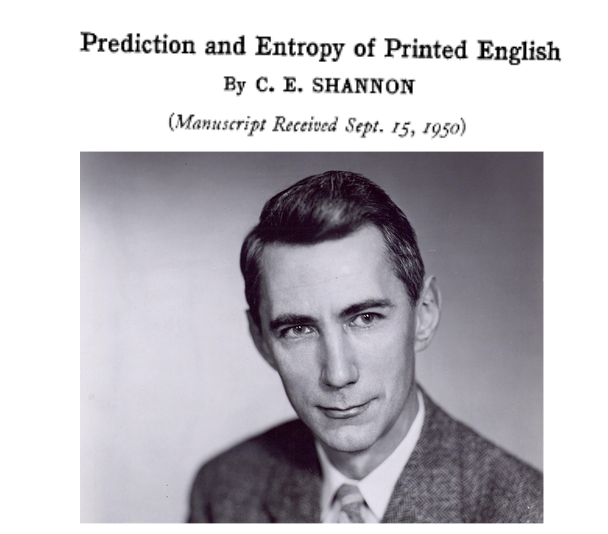
\includegraphics[scale = 0.4]{pics/shannon.png}
    \caption{Imagen de Shannon.}
    \label{fig:shannon}
\end{figure}

Por otro lado, en su libro \textit{Syntactic Structures} (1957), Noam Chomsky (en la Figura~\ref{fig:chomsky}), un lingüista y científico cognitivo, cuestionó la capacidad de los modelos de lenguaje probabilísticos para capturar y comprender la gramática del lenguaje humano \cite{chomsky2009syntactic}. Según Chomsky, la noción de ``gramaticamente correcto'' no puede ser equiparada a ``significativo'' en un sentido probabilista. Para ilustrar esto, presentó dos oraciones ficticias, ambas carentes de sentido:

\begin{enumerate}
    \item Colorless green ideas sleep furiously.
    \item Furiously sleep ideas green colorless.
\end{enumerate}

Aunque ambas oraciones carecen de significado, Chomsky argumentó que solo la primera se considera gramaticalmente correcta por los hablantes de inglés. Además, enfatizó que la corecctitud gramatical en inglés no puede determinarse únicamente mediante aproximaciones estadísticas. Aunque es poco probable que ninguna de las dos oraciones (1) o (2) haya surgido en documentos escritos en inglés, un modelo estadístico como los modelos de lenguaje vistos en este capítulo las consideraría igualmente ``remotas'' en relación al inglés. Sin embargo, la oración (1) es gramaticalmente correcta, mientras que la oración (2) no lo es, lo que destaca las limitaciones de los enfoques estadísticos para capturar la gramática. Estos argumentos retrasaron el estudio de los modelos de lenguaje probabilísticos durante varios años \cite{JurafskyBook}.

\begin{figure}[h]
    \centering
    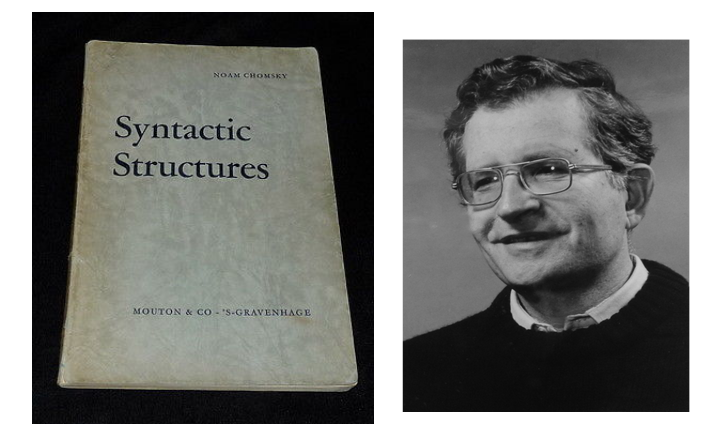
\includegraphics[scale = 0.4]{pics/chomsky.png}
    \caption{Imagen de Chomsky}
    \label{fig:chomsky}
\end{figure}


\section{Conclusiones}
La derivación de probabilidades en modelos de lenguaje probabilísticos implica tres pasos:
    \begin{enumerate}
        \item Expandir $p(w_1, w_2, \ldots, w_n)$ usando la regla de la Cadena.
        \item Aplicar las Asunciones de Independencia de Markov \\
        $p(w_i | w_1, w_2, \ldots, w_{i-2}, w_{i-1}) = p(w_i | w_{i-2}, w_{i-1})$.
        \item Suavizar las estimaciones utilizando conteos de orden inferior.
    \end{enumerate}
Otros métodos para mejorar los modelos de lenguaje incluyen introducir variables latentes para representar tópicos, conocidos como modelos de tópicos \cite{blei2003latent} presentados en el Capítulo~\ref{cap_ir}. O alternativamente, reemplazar $p(w_i | w_1, w_2, \ldots, w_{i-2}, w_{i-1})$ con una red neuronal predictiva y una ``capa de embedding'' para representar mejor contextos más grandes y aprovechar similitudes entre palabras en el contexto. \cite{bengio2000neural}

Los modelos de lenguaje modernos utilizan redes neuronales profundas en su estructura principal y tienen un vasto espacio de parámetros como se verá en el Capítulo~\ref{cap_llm}.

